\documentclass[11pt,a4paper]{article}

\usepackage[utf8]{inputenc}
\usepackage[T1]{fontenc}
\usepackage{mathpazo}
\usepackage[scaled=0.92]{helvet}
\usepackage[margin=1in]{geometry}
\usepackage{graphicx}
\usepackage{amsmath,amssymb,amsfonts}
\usepackage{booktabs}
\usepackage{tabularx}
\usepackage{setspace}
\usepackage{titlesec}
\usepackage{fancyhdr}
\usepackage{float}
\usepackage{caption}
\usepackage{microtype}

\usepackage{tikz}
\usetikzlibrary{shapes.geometric, arrows.meta, positioning, calc}

\usepackage{listings}
\usepackage{xcolor}
\usepackage[hidelinks]{hyperref}

% --- SETUP (Sesuai dengan Paper Anda) ---
\setstretch{1.15}
\setlength{\parindent}{0pt}
\setlength{\parskip}{0.8em}
\sloppy

\titleformat{\section}{\normalfont\large\bfseries\sffamily}{\thesection}{1em}{}
\titleformat{\subsection}{\normalfont\normalsize\bfseries\sffamily}{\thesubsection}{1em}{}

\pagestyle{fancy}
\fancyhf{}
\fancyhead[L]{\small\sffamily Fondasi Basis Data: Normalisasi}
\fancyhead[R]{\small\sffamily\thepage}
\renewcommand{\headrulewidth}{0.4pt}

\captionsetup{font=small,labelfont=bf,labelsep=period}

\renewenvironment{abstract}
{\small
	\begin{center}\textbf{\sffamily Abstrak}\end{center}
	\begin{quote}}
	{\end{quote}}

\title{\vspace{-1.5cm}\textbf{\sffamily\LARGE Fondasi Basis Data: Normalisasi dan Anomali}}
\author{
	\textbf{Muhammad Riduwan Khafidi} \\
	\small Program Studi Teknik Rekayasa Perangkat Lunak \\
	\small Politeknik Negeri Batam \\
	\small \texttt{4342611034@students.polibatam.ac.id}
}
\date{\small\today}

\begin{document}

\maketitle
\thispagestyle{empty}

\begin{abstract}
	Normalisasi adalah teknik fundamental dalam desain logis basis data yang bertujuan untuk mengelompokkan atribut ke dalam tabel-tabel agar terbentuk struktur relasi yang baik, efisien, dan bebas dari redundansi. Tanpa normalisasi, basis data rentan terhadap tiga masalah utama yang disebut Anomali: Anomali Peremajaan (Update), Penyisipan (Insert), dan Penghapusan (Delete). Makalah ini membahas konsep dasar dependensi fungsional, proses dekomposisi tabel, serta tahapan bentuk normal (1NF, 2NF, 3NF, dan BCNF) dengan pendekatan studi kasus.
\end{abstract}

\section{Pendahuluan}

Basis data yang tidak dirancang dengan baik akan mengalami redundansi data (pengulangan data yang sama di banyak tempat). Hal ini tidak hanya memboroskan ruang penyimpanan, tetapi juga memicu terjadinya anomali, yaitu efek samping yang tidak diharapkan saat data dimanipulasi. Normalisasi hadir sebagai proses dekomposisi tabel untuk mengurangi redundansi dan memastikan integritas data tetap terjaga.

\section{Tiga Jenis Anomali}

Jika sebuah tabel tidak dinormalisasi, akan muncul tiga jenis anomali yang dapat merusak konsistensi data:

\begin{enumerate}
	\item \textbf{Anomali Peremajaan (Update Anomaly):} Terjadi ketika sebuah data diubah pada satu baris, tetapi tidak diubah pada baris lain yang memiliki data sama, sehingga menimbulkan inkonsistensi.
	\item \textbf{Anomali Penyisipan (Insert Anomaly):} Terjadi ketika kita tidak dapat menambahkan data baru karena ada elemen lain (yang menjadi kunci) belum tersedia. Hal ini sering disebabkan oleh atribut yang dipaksakan dalam satu tabel.
	\item \textbf{Anomali Penghapusan (Delete Anomaly):} Terjadi ketika penghapusan satu baris data secara tidak sengaja juga menghapus data lain yang masih relevan dan penting.
\end{enumerate}

\subsection{Ilustrasi Kasus Anomali}

Perhatikan tabel \textbf{Pesanan} yang belum dinormalisasi berikut ini:

\begin{table}[H]
	\centering
	\small
	\caption{Tabel Pesanan (Belum Ternormalisasi)}
	\begin{tabularx}{0.7\textwidth}{@{} l l l c @{}}
		\toprule
		\textbf{Pemasok} & \textbf{Kota} & \textbf{Barang} & \textbf{Jumlah} \\
		\midrule
		Kartika          & Jakarta       & Mouse           & 5               \\
		Citra            & Bandung       & Monitor         & 2               \\
		Yudi             & Medan         & CPU             & 2               \\
		Citra            & Bandung       & Printer         & 1               \\
		\bottomrule
	\end{tabularx}
\end{table}

Dari tabel di atas, dapat diidentifikasi permasalahan sebagai berikut:
\begin{itemize}
	\item Jika Citra pindah domisili dari Bandung ke Bogor, perubahan harus dilakukan pada dua baris. Jika hanya satu baris yang diubah, data menjadi tidak konsisten (Anomali Update).
	\item Jika pesanan Monitor dihapus, dan itu satu-satunya pesanan dari Citra, maka informasi bahwa Citra adalah pemasok akan hilang dari sistem (Anomali Delete).
	\item Jika terdapat pemasok baru yang belum melakukan pemesanan, data pemasok tersebut tidak dapat dimasukkan karena kolom Barang dan Jumlah harus terisi (Anomali Insert).
\end{itemize}

\section{Dependensi Fungsional}

Dependensi fungsional (\textit{Functional Dependency}) adalah hubungan antara dua atribut di mana nilai satu atribut menentukan nilai atribut lainnya secara unik. Notasi yang digunakan adalah \(X \rightarrow Y\) (X menentukan Y).

\begin{figure}[H]
	\centering
	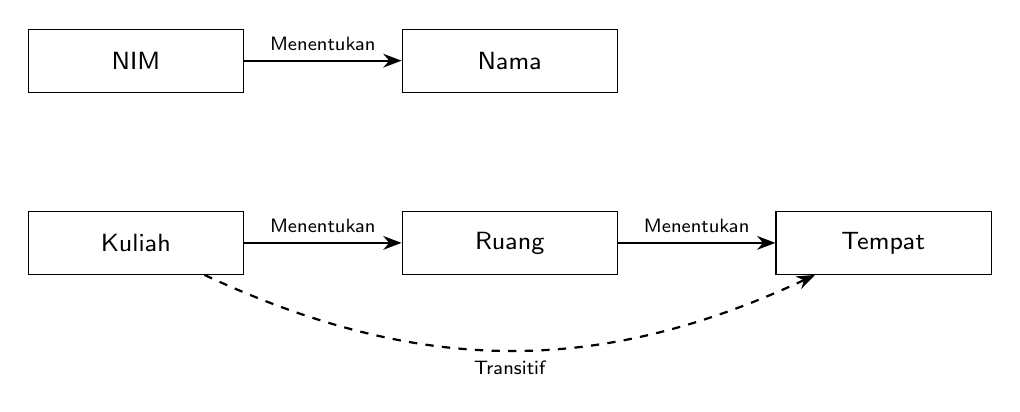
\begin{tikzpicture}[
			node distance=1.5cm and 2cm,
			box/.style={rectangle, draw=black, thin, text width=2.5cm, align=center, minimum height=0.8cm, font=\sffamily\small},
			arrow/.style={->, >=Stealth, thick, color=black}
		]
		% Dependensi Normal
		\node[box] (nim) {NIM};
		\node[box, right=2cm of nim] (nama) {Nama};
		\draw[arrow] (nim) -- node[above, font=\scriptsize\sffamily] {Menentukan} (nama);

		% Dependensi Transitif
		\node[box, below=1.5cm of nim] (kuliah) {Kuliah};
		\node[box, right=2cm of kuliah] (ruang) {Ruang};
		\node[box, right=2cm of ruang] (tempat) {Tempat};

		\draw[arrow] (kuliah) -- node[above, font=\scriptsize\sffamily] {Menentukan} (ruang);
		\draw[arrow] (ruang) -- node[above, font=\scriptsize\sffamily] {Menentukan} (tempat);
		\draw[arrow, dashed] (kuliah) to[bend right=25] node[below, font=\scriptsize\sffamily] {Transitif} (tempat);
	\end{tikzpicture}
	\caption{Ilustrasi Dependensi Fungsional Biasa dan Transitif.}
\end{figure}

\section{Tahapan Bentuk Normalisasi}

\subsection{First Normal Form (1NF)}
Aturan 1NF mengharuskan semua atribut bersifat atomik. Tidak boleh ada atribut yang memiliki nilai ganda (\textit{multivalued}) atau kelompok data berulang dalam satu sel.

\begin{table}[H]
	\centering
	\small
	\caption{Transformasi dari Unnormalized ke 1NF}
	\begin{tabularx}{\textwidth}{@{} X X @{}}
		\toprule
		\textbf{Unnormalized (Salah)} & \textbf{1NF (Benar)} \\
		\midrule
		\begin{tabular}[t]{@{}lll@{}}
			\toprule
			NIM & Nama  & Keahlian      \\
			\midrule
			107 & Ilham & Cobol, Oracle \\
			120 & Fika  & Dbase, Sybase \\
			\bottomrule
		\end{tabular}
		                              &
		\begin{tabular}[t]{@{}lll@{}}
			\toprule
			NIM & Nama  & Keahlian \\
			\midrule
			107 & Ilham & Cobol    \\
			107 & Ilham & Oracle   \\
			120 & Fika  & Dbase    \\
			120 & Fika  & Sybase   \\
			\bottomrule
		\end{tabular}                         \\
		\bottomrule
	\end{tabularx}
\end{table}

\subsection{Second Normal Form (2NF)}
Aturan 2NF mengharuskan tabel sudah dalam bentuk 1NF dan tidak memiliki ketergantungan parsial (\textit{partial dependency}). Ketergantungan parsial hanya terjadi jika tabel memiliki \textit{Composite Primary Key} (Kunci Utama gabungan).

\textbf{Masalah:} Pada tabel \texttt{Nilai (NIM, KodeMK, NamaMhs, NilaiAkhir)}, kunci utamanya adalah \texttt{(NIM, KodeMK)}. Namun, atribut \texttt{NamaMhs} hanya bergantung pada \texttt{NIM} saja, sehingga melanggar aturan 2NF.

\textbf{Solusi:} Tabel dipecah menjadi dua:
\begin{itemize}
	\item Tabel \texttt{Mahasiswa (NIM, NamaMhs)}
	\item Tabel \texttt{Nilai (NIM, KodeMK, NilaiAkhir)}
\end{itemize}

\subsection{Third Normal Form (3NF)}
Aturan 3NF mengharuskan tabel sudah dalam bentuk 2NF dan tidak memiliki ketergantungan transitif (\textit{transitive dependency}). Artinya, atribut non-kunci tidak boleh bergantung pada atribut non-kunci lainnya.

\textbf{Masalah:} Pada tabel \texttt{Kuliah (Kuliah, Ruang, Tempat, Waktu)}, terdapat dependensi \texttt{Kuliah \(\rightarrow\) Ruang} dan \texttt{Ruang \(\rightarrow\) Tempat}. Hal ini menyebabkan \texttt{Tempat} bergantung secara transitif pada \texttt{Kuliah}.

\textbf{Solusi:} Tabel dipecah menjadi dua:
\begin{itemize}
	\item Tabel \texttt{Ruangan (Ruang, Tempat)}
	\item Tabel \texttt{Jadwal (Kuliah, Ruang, Waktu)}
\end{itemize}

\subsection{Boyce-Codd Normal Form (BCNF)}
BCNF adalah bentuk yang lebih ketat dari 3NF. Aturannya adalah setiap atribut penentu (\textit{determinant}) harus merupakan \textit{Candidate Key}. BCNF menyelesaikan kasus anomali yang tidak dapat diselesaikan oleh 3NF, umumnya terjadi ketika terdapat dua \textit{Candidate Key} yang saling tumpang tindih.

\section{Studi Kasus Normalisasi}

Diberikan tabel hasil rekapitulasi nilai mahasiswa yang belum dinormalisasi sebagai berikut:

\begin{table}[H]
	\centering
	\small
	\caption{Tabel Unnormalized (UNF)}
	\begin{tabularx}{\textwidth}{@{} l l l l l c @{}}
		\toprule
		\textbf{NIM} & \textbf{NamaMhs} & \textbf{Jurusan} & \textbf{KodeMK} & \textbf{NamaMK} & \textbf{Nilai} \\
		\midrule
		2683         & Willi            & MI               & MI350           & Manajemen SI    & A              \\
		2683         & Willi            & MI               & MI240           & Basis Data      & B              \\
		5432         & Bakri            & AK               & AK201           & Akuntansi Dasar & A              \\
		\bottomrule
	\end{tabularx}
\end{table}

\textbf{Langkah 1: Uji 1NF} \\
Tabel di atas telah memenuhi syarat 1NF karena setiap sel hanya berisi satu nilai atomik.

\textbf{Langkah 2: Uji 2NF} \\
Kunci utama dari tabel tersebut adalah \texttt{\{NIM, KodeMK\}}. Terdapat ketergantungan parsial:
\begin{itemize}
	\item \texttt{NamaMhs} dan \texttt{Jurusan} hanya bergantung pada \texttt{NIM}.
	\item \texttt{NamaMK} hanya bergantung pada \texttt{KodeMK}.
\end{itemize}
Maka, dekomposisi tabel dilakukan untuk menghilangkan ketergantungan parsial:

\begin{table}[H]
	\centering
	\small
	\caption{Hasil Dekomposisi 2NF}
	\begin{tabularx}{\textwidth}{@{} X X X @{}}
		\toprule
		\textbf{Mahasiswa} & \textbf{MataKuliah} & \textbf{Nilai} \\
		\midrule
		\begin{tabular}[t]{@{}lll@{}}
			\toprule
			NIM  & Nama  & Jurusan \\
			\midrule
			2683 & Willi & MI      \\
			5432 & Bakri & AK      \\
			\bottomrule
		\end{tabular}
		                   &
		\begin{tabular}[t]{@{}ll@{}}
			\toprule
			Kode  & NamaMK          \\
			\midrule
			MI350 & Manajemen SI    \\
			MI240 & Basis Data      \\
			AK201 & Akuntansi Dasar \\
			\bottomrule
		\end{tabular}
		                   &
		\begin{tabular}[t]{@{}llc@{}}
			\toprule
			NIM  & KodeMK & Nilai \\
			\midrule
			2683 & MI350  & A     \\
			2683 & MI240  & B     \\
			5432 & AK201  & A     \\
			\bottomrule
		\end{tabular}                              \\
		\bottomrule
	\end{tabularx}
\end{table}

\textbf{Langkah 3: Uji 3NF} \\
Pemeriksaan dilakukan pada ketiga tabel hasil dekomposisi. Tidak ditemukan adanya atribut non-kunci yang bergantung pada atribut non-kunci lainnya. Dengan demikian, skema relasional tersebut telah memenuhi bentuk normal ketiga (3NF) dan siap diimplementasikan.

\section{Kesimpulan}

Normalisasi merupakan proses penting dalam perancangan basis data untuk memastikan data tersimpan secara efisien dan konsisten. Prinsip utamanya adalah memastikan setiap atribut non-kunci hanya bergantung pada kunci utamanya. Penerapan 1NF, 2NF, 3NF, dan BCNF secara berurutan akan menghilangkan anomali data dan menghasilkan struktur basis data yang siap digunakan untuk aplikasi berskala besar.

\newpage
\section*{Referensi}
\addcontentsline{toc}{section}{Referensi}

\begin{thebibliography}{99}
	\bibitem{slide}
	Mardiani, G. T. (n.d.). \textit{Normalisasi Basis Data} [Slide Presentasi Mata Kuliah Basis Data].

	\bibitem{binus}
	BINUS University. (2022). \textit{Normalisasi}. School of Information Systems.

	\bibitem{silberschatz}
	Silberschatz, A., Korth, H. F., \& Sudarshan, S. (2019). \textit{Database System Concepts} (7th ed.). McGraw-Hill Education.
\end{thebibliography}

\end{document}
